%% 
%% Copyright 2007-2020 Elsevier Ltd
%% 
%% This file is part of the 'Elsarticle Bundle'.
%% ---------------------------------------------
%% 
%% It may be distributed under the conditions of the LaTeX Project Public
%% License, either version 1.2 of this license or (at your option) any
%% later version.  The latest version of this license is in
%%    http://www.latex-project.org/lppl.txt
%% and version 1.2 or later is part of all distributions of LaTeX
%% version 1999/12/01 or later.
%% 
%% The list of all files belonging to the 'Elsarticle Bundle' is
%% given in the file `manifest.txt'.
%% 
%% Template article for Elsevier's document class `elsarticle'
%% with harvard style bibliographic references

%\documentclass[preprint,12pt,authoryear]{elsarticle}

%% Use the option review to obtain double line spacing
%% \documentclass[authoryear,preprint,review,12pt]{elsarticle}

%% Use the options 1p,twocolumn; 3p; 3p,twocolumn; 5p; or 5p,twocolumn
%% for a journal layout:
%% \documentclass[final,1p,times,authoryear]{elsarticle}
%% \documentclass[final,1p,times,twocolumn,authoryear]{elsarticle}
%% \documentclass[final,3p,times,authoryear]{elsarticle}
%% \documentclass[final,3p,times,twocolumn,authoryear]{elsarticle}
%% \documentclass[final,5p,times,authoryear]{elsarticle}
 \documentclass[final,5p,times,twocolumn,authoryear, 12pt]{elsarticle}

 


%% For including figures, graphicx.sty has been loaded in
%% elsarticle.cls. If you prefer to use the old commands
%% please give \usepackage{epsfig}

%% The amssymb package provides various useful mathematical symbols
\usepackage{amssymb}
\usepackage{lipsum}
\usepackage{wrapfig}
\usepackage{changepage}
\usepackage{setspace}

%% The amsthm package provides extended theorem environments
%% \usepackage{amsthm}

%% The lineno packages adds line numbers. Start line numbering with
%% \begin{linenumbers}, end it with \end{linenumbers}. Or switch it on
%% for the whole article with \linenumbers.
%% \usepackage{lineno}

%% You might want to define your own abbreviated commands for common used terms, e.g.:
\newcommand{\kms}{km\,s$^{-1}$}
\newcommand{\msun}{$M_\odot}


\setstretch{1.25}

\begin{document}

\begin{frontmatter}

%% Title, authors and addresses

%% use the tnoteref command within \title for footnotes;
%% use the tnotetext command for theassociated footnote;
%% use the fnref command within \author or \affiliation for footnotes;
%% use the fntext command for theassociated footnote;
%% use the corref command within \author for corresponding author footnotes;
%% use the cortext command for theassociated footnote;
%% use the ead command for the email address,
%% and the form \ead[url] for the home page:
%% \title{Title\tnoteref{label1}}
%% \tnotetext[label1]{}
%% \author{Name\corref{cor1}\fnref{label2}}
%% \ead{email address}
%% \ead[url]{home page}
%% \fntext[label2]{}
%% \cortext[cor1]{}
%% \affiliation{organization={},
%%            addressline={}, 
%%            city={},
%%            postcode={}, 
%%            state={},
%%            country={}}
%% \fntext[label3]{}

\title{\bf ORIE 4741 Final Report: S\&P 500 Predictor}

%% use optional labels to link authors explicitly to addresses:
%% \author[label1,label2]{}
%% \affiliation[label1]{organization={},
%%             addressline={},
%%             city={},
%%             postcode={},
%%             state={},
%%             country={}}
%%
%% \affiliation[label2]{organization={},
%%             addressline={},
%%             city={},
%%             postcode={},
%%             state={},
%%             country={}}

\author{Trey Hensel (sch86), Jasper Hsu (jkh223), Thomas Suman (tcs97)}


\begin{abstract}
%% Text of abstract
The S\&P500 is a benchmark for the United States stock market, and its value is closely monitored by investors, financial analysts, and policymakers. Predicting the future value of the S\&P 500 SPY can help investors make informed decisions about buying or selling stocks, optimize their investment portfolios, and manage their risk exposure. This project uses machine learning techniques to predict the future value of the S\&P500, specifically techniques such as linear regression and classification. We also employ different loss functions, regularizers, feature transformations, and kernels in order to improve the generalization of the models. We then analyze the success and limitations of the model.

\end{abstract}

%%Graphical abstract
%\begin{graphicalabstract}
%\includegraphics{grabs}
%\end{graphicalabstract}

%%Research highlights
%\begin{highlights}
%\item Research highlight 1
%\item Research highlight 2
%\end{highlights}




\end{frontmatter}

%\tableofcontents

%% \linenumbers

%% main text

\section{Introduction}
\label{introduction}

\subsection{Background}


The S\&P 500, short for the Standard \& Poor's 500 Index, is a market-capitalization-weighted index of the 500 largest publicly traded companies in the United States. The index is widely regarded as a benchmark for the performance of the overall U.S. stock market and is used as a barometer for the health of the U.S. economy. Companies included in the S\&P 500 span across various industries and sectors, providing a diverse representation of the U.S. economy. The index is frequently used by investors, analysts, and economists to track market trends and evaluate investment opportunities. Understanding the S\&P 500 is essential for anyone interested in finance, investing, or the stock market.

\subsection{Problem Statement}

The purpose of this project is to develop a predictive model that can accurately forecast the value of the S\&P 500. To achieve this goal, the project will focus on predicting specific features of the S\&P 500, such as open price, close price, high price, low price, and volume. These features are key indicators of the overall market trends and are critical for making informed investment decisions. Open and close prices provide insight into market sentiment and investor behavior, while high and low prices reflect the overall volatility and risk associated with the market. Volume measures the total number of shares traded in a given time frame and can indicate the level of market participation or interest. By analyzing these features and developing a predictive model, the project aims to provide valuable insights into the future performance of the S\&P 500, ultimately helping investors make informed investment decisions.

\section{Data Analysis}
%%\label{}
\subsection{Dataset}

The S\&P 500 dataset available on Kaggle provides a comprehensive collection of historical price and volume data for the SPDR S\&P 500 ETF Trust (SPY), an exchange-traded fund that tracks the performance of the S\&P 500 index. The dataset includes daily information spanning from January 1993 to March 2023, providing over 7500 data points to analyze.
The dataset contains 10 numerical features/columns, including the open price, high price, low price, close price, and volume, and 1 ordinal date column. The open, high, low, and close prices provide insight into the daily market trends and investor behavior, while the volume measures the total number of shares traded on a given day.

\subsection{Data Cleaning}

To use the dataset for regression analysis, we needed to convert the "Date" column, which was in ordinal string format, to integer numerical values. We used a times-to-timestamp function to perform this conversion, which allowed us to easily manipulate and analyze the date values in our regression model. This conversion enabled us to capture the temporal aspect of the data and incorporate it into our predictive model accurately.

\subsection{Feature Engineering}

In addition to cleaning the data, we also had to transform the data to build certain models. These models would help us identify trends in the data that we previously did not have access to with the raw data. We will go into more depth later in this paper, but some examples of this feature engineering include plugging our data into a transformation function and moving certain data to new rows to reflect the knowledge we would have at a given time period.

% HOW TO ADD AN IMAGE IS RIGHT HERE 

% \begin{figure}
% 	\centering 
% 	
\includegraphics[width=0.4\textwidth, angle=-90]{ASCOM_journal_cover.pdf}	
% 	\caption{Astronomy \& Computing journal cover} 
% 	\label{fig_mom0}%
% \end{figure}



\section{Model Approach: Linear Regression}
%%\label{}
    We aim to predict the closing price of the S\&P 500 on any given day. A regression model best suits this problem because, given an input vector, it predicts the most likely numerical value. We will explore different regression models and techniques throughout this paper in order to produce the best possible results.
    

\subsection{Linear Regression with Ordinary Least Squares}


	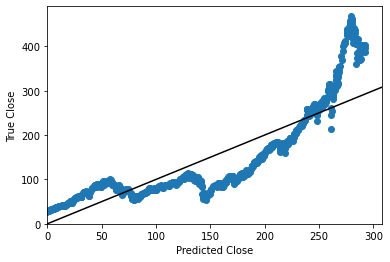
\includegraphics[width=0.4\textwidth, angle=0]{linregOLS.png}	

In our first attempt to model the S\&P 500, we decided to predict the closing value using the date. We used ordinary least squares regression, which has the following objective function:

\begin{adjustwidth}{1.6cm}{}
\[
   \arg \min_w \frac{1}{n} \sum_{i = 1}^{n} (y_i - w^T x_i)^2
\]
\end{adjustwidth}

Learning the model resulted in a train mean square error (MSE) of 2756.120 and a test MSE of 2904.999. Additionally, the time coefficient is 33.087, and the intercept is -262.017. The observed MSE values imply that the model's predictive accuracy may be inadequate for practical purposes. Additionally, the R-squared value of 0.747 suggests that the model explains about 74.7\% of the variability in the dependent variable, leaving a significant portion unexplained. Possible reasons for this include the lack of important predictor variables or the presence of nonlinear relationships between the close values and the date. Further analysis and improvement of the model is necessary to achieve better predictive accuracy.

\subsection{Ridge Regression}

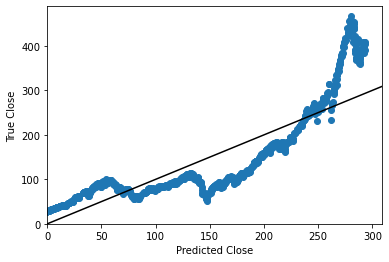
\includegraphics[width=0.4\textwidth, angle=0]{linregRR.png}

After performing ordinary least squares regression on the data, we decided to add a regularizer to the data. This allows us to prevent overfitting by increasing the error when w gets large.


\begin{adjustwidth}{1cm}{}
    \[ \arg \min_w \frac{1}{n} \sum_{i = 1}^{n} (y_i - w^T x_i)^2 + r(w)\]
\end{adjustwidth}

\begin{adjustwidth}{2.1cm}{}
        \[r(w) = \lambda\sum_{i=1}^d w_i^2\]

\end{adjustwidth}

We started off with ridge regression, which means that we define $r(w)$ as it is defined above. However, we found that adding this regularizer had virtually no effect. Our training MSE came out to be 2756.120 and our test MSE is 2905.007, so both our errors change by less than 0.01. We determined that this is a result of our model choosing a low w and the intercept having a small affect on the data. Through this model, our intercept term gets pushed down to 0, while our time variable is almost the same as before. So, we decided that since our w is small and likely doesn't overfit the data, we decided that we would not look at other regularizers because they would likely not have big effects.

\subsection{Linear Regression with Huber Loss}

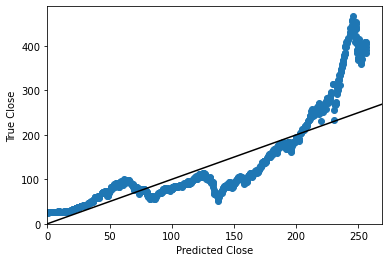
\includegraphics[width=0.4\textwidth, angle=0]{linregHuber.png}

In order to improve our model, we decided to investigate using different loss functions. One loss function we tried to use was the Huber loss function.  The objective function of linear regression with Huber loss is defined as:

\begin{adjustwidth}{1cm}{}
    \[
        \arg \min_w \frac{1}{n} \sum_{i = 1}^{n} \textbf{huber}(y_i - w^T x_i)
    \]
\end{adjustwidth}

This function is a robust loss function, which means that it is less sensitive to outliers. So, we thought it would be interesting to use this function to see if the outliers in this dataset were causing the error. After learning the new model, we obtained a training MSE of 3078.050 and a test MSE of 3358.484. It is evident that the Huber loss model performs worse than the OLS model. However, the loss was not that far off form OLS so we decided to try another robust loss function to get a better sense of how the model reacts to the outliers.

\subsection{Linear Regression with Quantile Loss}

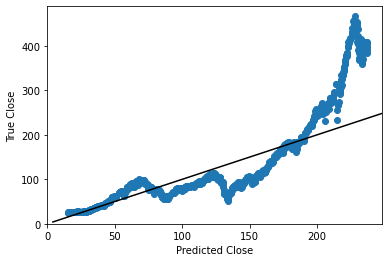
\includegraphics[width=0.4\textwidth, angle=0]{linregQ.png}		

Another loss function that we used was the quantile loss function. This is an additional type of a robust loss function. It is defined as 

\begin{adjustwidth}{1.4cm}{}
    \[
        \arg \min_w \frac{1}{n} \sum_{i = 1}^{n} \alpha (y_i - w^Tx_i)^+
    \]
\end{adjustwidth}
\begin{adjustwidth}{2.0cm}{}
    \[
        + (1 - \alpha) (y_i - w^Tx_i)^-
    \]
\end{adjustwidth}

We see a similar outcome when using this loss function. We get a training MSE of 3542.257 and a test MSE of 3884.462. This loss does a significantly worse job than OLS. So, we concluded that the outliers were not one of our main issues.

\subsection{Linear Regression with Feature Transformation}

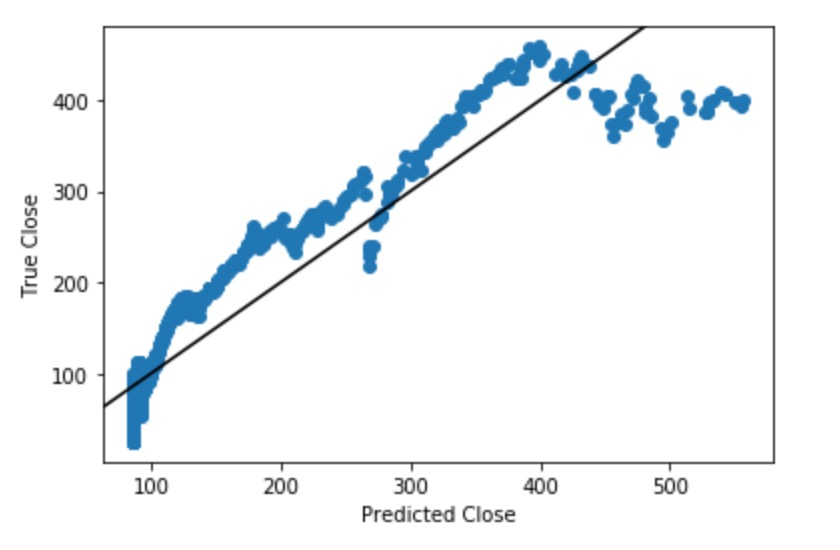
\includegraphics[width=0.4\textwidth, angle=0]{linregFT.jpeg}

After performing our regression analysis with different kinds of loss functions, we used feature engineering as another way to try to gain more insight from the data. Through research and prior knowledge, we knew that stock prices over time can approximately be modeled through an exponential function. So, we used our function

\begin{adjustwidth}{2.8cm}{}
    \[
        \phi(t) = e^t
    \]
\end{adjustwidth}

This function takes time as our input parameter and outputs the exponential of the time. This allowed us to transform our data into a new dataset that would eventually help us see a more linear relationship within the data points. As shown in the graph, our predictions do a much better job of accurately forecasting the true close price. Additionally, this model lowers our training MSE to 1581.530 and our test MSE to 1615.756. This model is definitely a step in the right direction and led us to pursue the model in our next section.

\subsection{Kernel Regression}

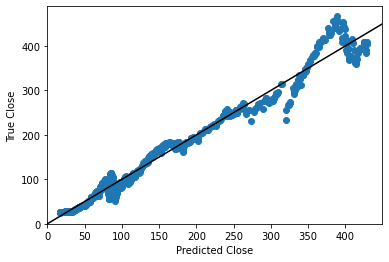
\includegraphics[width=0.4\textwidth, angle=0]{linregRBF.png}




After considering the results from the different linear regression models and the significant improvement made with the feature engineering transformation, it was evident that our data exhibits a nonlinear trend. As such, we decided to use kernelized regression, in order to learn a nonlinear regression curve to better predict the value of the S\&P500 on a given day. By applying a kernel function, the data is implicitly mapped into a higher-dimensional feature space where linear regression can be performed. This enables the model to capture complex patterns and nonlinear dependencies that a standard linear regression cannot handle. Specifically, we thought that the Radial Basis Function (RBF) kernel, which uses the Gaussian density, would be a good kernel function because of its relationship with our transformation function from the Feature Engineering section. The RBF kernel is one of the most popular and universal kernels. It is defined as:

\begin{adjustwidth}{1.8cm}{}
    \[K(x, x') = e^{- \frac{||x - x'||^2}{2\sigma^2}} \]
\end{adjustwidth}

This kernel function works by calculating the similarity of a pair of two data points, which is a function of the Euclidean distance between the two points. It then stores this as a new feature, increasing the dimensionality of the data. This is done for each possible pair consisting of a new data point and an existing training point. Then, these new features are used in order to predict the regression value for the new data point. It can be seen in the graph that this is our best predictor. The relationship between the true closing price and the predicted closing price in the higher dimensional transformation is clearly linear, with a bit of noise and inaccuracy. 

After learning the RBF kernelized regression model, we achieved a training MSE of 301.758 and a test MSE of 297.483. This is far lower than the error from any of the other models we have implemented previously. This implies that the model is able to capture the underlying patterns and relationships in the training data effectively. The low train error indicates that the model has learned the training examples well, while the low test error suggests that it generalizes well to unseen data. This implies that the model is a good fit for the data, and it can accurately predict the target variable for new instances. This also suggests that the model's complexity is appropriate for the data. These conclusions suggest that the model is reliable and can be used for accurate predictions on new data.




% hOW TO DO A TABLE

% \begin{table}
% \begin{tabular}{l c c c} 
%  \hline
%  Source & RA (J2000) & DEC (J2000) & $V_{\rm sys}$ \\ 
%         & [h,m,s]    & [o,','']    & \kms          \\
%  \hline
%  NGC\,253 & 	00:47:33.120 & -25:17:17.59 & $235 \pm 1$ \\ 
%  M\,82 & 09:55:52.725, & +69:40:45.78 & $269 \pm 2$ 	 \\ 
%  \hline
% \end{tabular}
% \caption{Random table with galaxies coordinates and velocities, Number the tables consecutively in
% accordance with their appearance in the text and place any table notes below the table body. Please avoid using vertical rules and shading in table cells.
% }
% \label{Table1}
% \end{table}


\section{Model Approach: Classification}

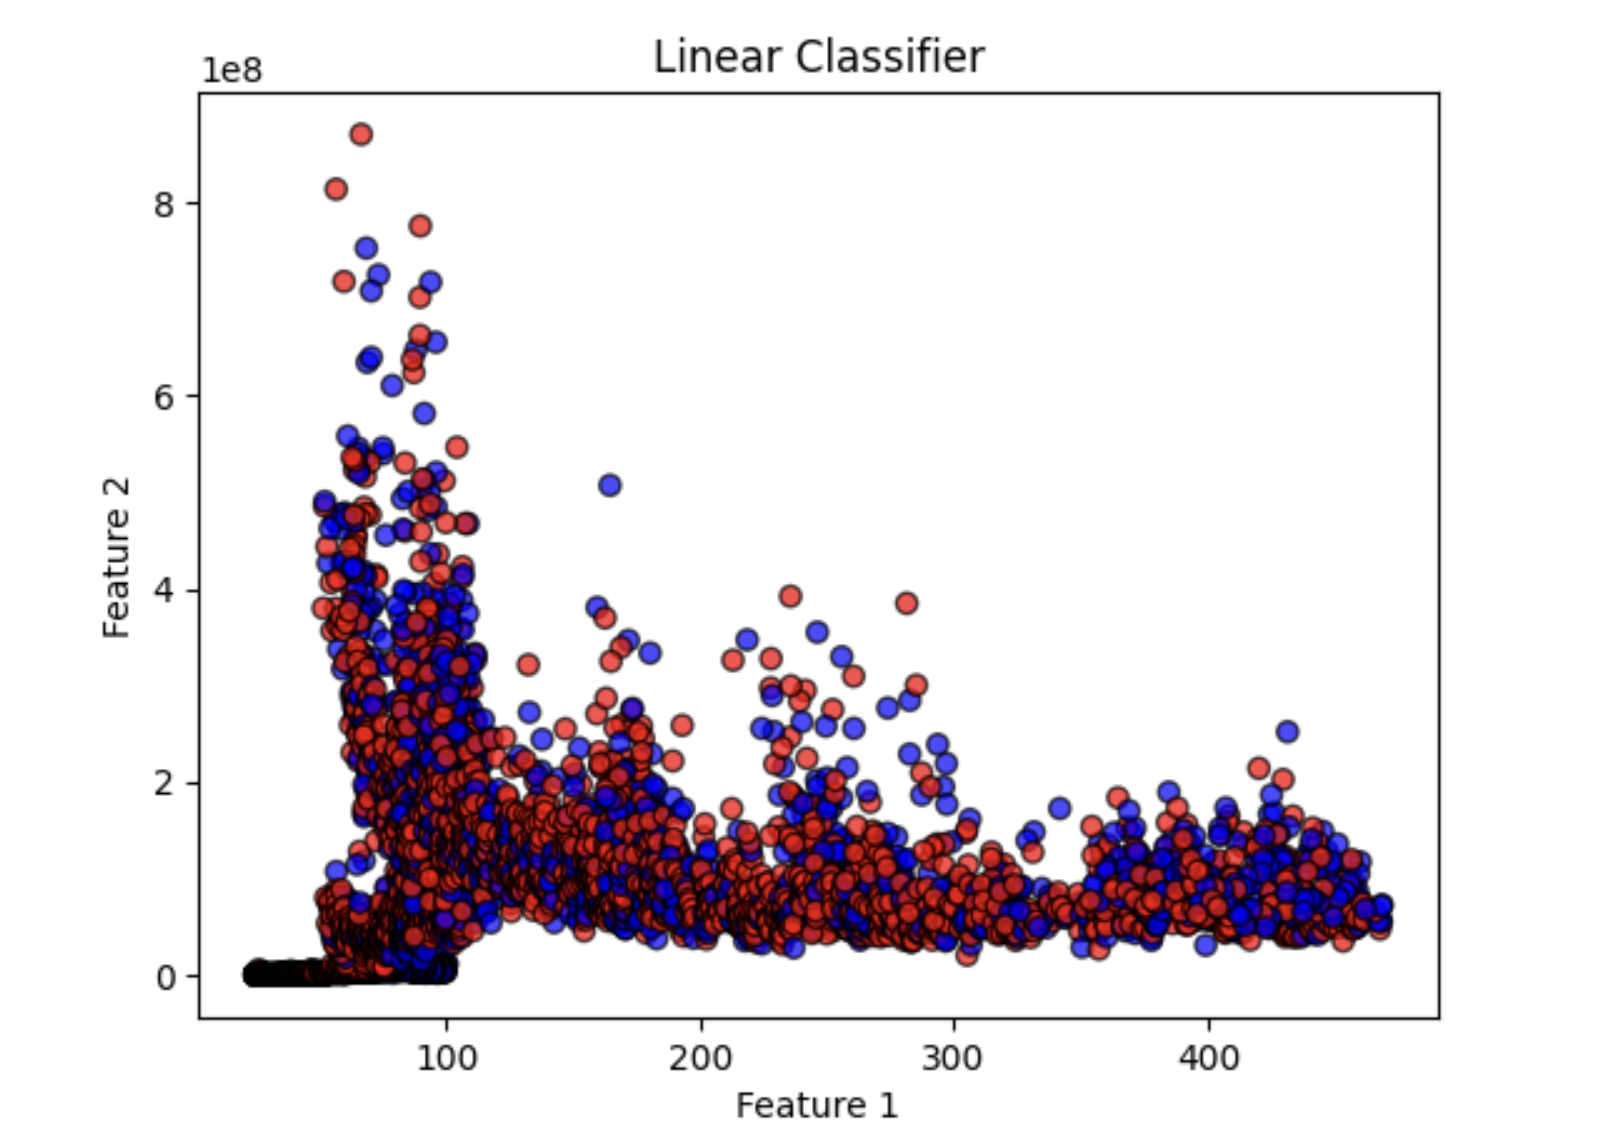
\includegraphics[width=0.4\textwidth, angle=0]{classification.png}

After investigating stock forecasting with regression, we looked to classify the stocks based on whether they go up or down. We wanted to use all of the knowledge up to a point in time in order to predict the direction of the stock's movement the next day. So, we used the two biggest factors: yesterday's price and yesterday's volume traded. The factors are plotted above, along with their classifications, where red signifies the stock went up and blue meaning the stock went down. These factors would show how much the stock would cost and how much demand there was for it. We wanted to plug these data points, along with their classifications, into the perceptron algorithm. This algorithm takes classified data points and splits them up into two groups by outputting a hyperplane that separates the the data by classification. However, it is necessary for the data to be linearly separable in order to implement the perceptron algorithm. As shown in the graph, it is visually obvious the data cannot be separated due to the massive overlap in the points. So, the perceptron algorithm is not able to find a hyperplane that separates the data and using the results from regression is a better way to make predictions.

\section{Summary and Conclusions}

In conclusion, this paper presents a project that aims to develop a predictive model for forecasting the value of the S\&P 500, based on specific features such as open, close, high, low prices, and volume. The dataset used in this project provides historical price and volume data from January 1993 to March 2023, and over 7500 data points have been analyzed. A linear regression approach using various loss functions and regularizers were used to model the S\&P 500 closing value using the date. However, the results obtained show that further analysis and improvement of the model is necessary to achieve better predictive accuracy. Thus, we employed a kernel linear regression approach and achieved better model accuracy. We used the Gaussian kernel to smooth the data and capture the underlying trend. The resulting model had a lower mean squared error and better overall performance than the previous linear regression models we employed. Our use of kernel regression demonstrates the importance of exploring different modeling techniques to achieve optimal results.

When considering whether this project could produce a "Weapon of Math Destruction," we need to assess whether the model satisfies the criteria of not easily measurable outcome, predictions with negative consequences, and self-fulfilling (or defeating) feedback loops. Although the S\&P 500 predictive model could have significant consequences for investors who use the forecast to make investment decisions, it is not clear whether the model could result in a WMD. The outcomes are easily measurable since the model predicts specific numerical values for the S\&P 500 features. However, the predictions can have negative consequences if investors rely solely on the model's predictions without considering other factors or market trends. Additionally, self-fulfilling feedback loops could be created if investors make decisions based on the model's predictions, which could ultimately affect the market's behavior.

When choosing a model for any application, including financial forecasting, fairness is an important criterion to consider. Fairness ensures that the model does not produce biased outcomes or perpetuate existing biases in the data. In this project, the fairness criterion was not explicitly considered, and it would be essential to assess whether the model produces unbiased results for all investors and stakeholders. A fair model ensures that investors can make informed investment decisions based on accurate predictions and reduces the potential for negative consequences.

To further improve the model and project, there are several steps that can be taken. Firstly, we could collect more data to increase the sample size and improve the robustness of the model. This could involve gathering additional data from different sources, or expanding the range of variables that are included in the analysis. Secondly, we could explore the use of more advanced machine learning techniques, such as neural networks or ensemble methods, to improve the accuracy of the model. These approaches can help to capture more complex relationships between the variables and may be particularly effective when dealing with high-dimensional data. Lastly, we could perform a more comprehensive evaluation of the model, using techniques such as cross-validation or sensitivity analysis, to assess its performance across different subsets of the data and under different assumptions. This would help to identify any weaknesses or limitations of the model, and guide further refinements and improvements.

\section{Contributions}

 All group members were involved in analyzing and cleaning the dataset, performing feature engineering, creating the first linear regression model using OLS, and the classification model attempt. Jasper Hsu took the lead on implementing models with different loss functions and regularizers, Trey Hensel lead the group in implementing the linear regression model with feature transformation, and Thomas Suman headed the implementation of the kernelized regression model, each of which with help from the other group members along the way. Finally, this project report is the result of the team working together to document their findings and analyze the different models.





%% The Appendices part is started with the command \appendix;
%% appendix sections are then done as normal sections


%% If you have bibdatabase file and want bibtex to generate the
%% bibitems, please use
%%


%% else use the following coding to input the bibitems directly in the
%% TeX file.

%%\begin{thebibliography}{00}

%% \bibitem[Author(year)]{label}
%% For example:

%% \bibitem[Aladro et al.(2015)]{Aladro15} Aladro, R., Martín, S., Riquelme, D., et al. 2015, \aas, 579, A101


%%\end{thebibliography}

\end{document}

\endinput
%%
%% End of file `elsarticle-template-harv.tex'.
